\subsection{Representative clustering: Basic notions}

Representative Clustering is about finding \emph{representatives} to cluster around, rather than the computationally expensive trying every single possible combination of possible clusters.

Examples are representative based clustering algorithms are
\begin{itemize}
    \item $k$-means (Each cluster is represented by its center)
    \item $k$-medoid (Each cluster is represented by one of its members)
\end{itemize}


\subsection{$k$-means clustering}
    \begin{defi}{$K$-means clustering}
        For a given $k$, form $k$ groups so that the sum of the squared distances between the mean of the groups (centroids) is minimal
    \end{defi}

Basic notions of $k$-means clustering are:
\begin{itemize}
    \item The objects $x = (x_1, \dots, x_d)$ are dots in a $d$-dimensional vector space where the main of the set is defined
    \item Centroids $\mu_C$ are the mean of the points in clustering $C$, where \m{
    \mu_C = \frac{1}{|C|}\sum_{x_j \in C}x_j
    }
    \item Measure for \emph{compactness} (Total distance) of a cluster $C_i$ \m{
    TD(C_i) = \sqrt{
    \sum_{x_j \in C_i}{dist(x_j, \mu_{C_{i}})^2}
    }
    }
    \item Measure for compactness of a \emph{clustering} \m{
        TD = \sqrt{\sum_{i=1}^{k}{TD^2(C_i)}}
    }. The ideal clustering minimizes this objective function.
    
\subsubsection{Lloyd's Algorithm}
    Lloyd's algorithm has 2 steps:
    First, partition into $k$ non-empty subsets
    \begin{enumerate}
        \item \textbf{Centroid update:} Compute centroids (Mean of cluster)
        \item \textbf{Cluster assignment:} Assign each object to cluster with nearest representative
    \end{enumerate}
    Repeat until represenatives do not change substantially. That means
    \m{
        \sum_{i=1}^{k} || \mu_i^t - \mu_i^{t-1}||^2 \leq \varepsilon
    }
\end{itemize}

\subsubsection{Advantages and disadvantages of $k$-means}
    The advantages are
    \begin{itemize}
        \item Efficient $O(tkn)$, where $n$ is number of points, $k$ is number of clusters and $t$ is number of iterations
        \item Normally $k, t$ is much smaller than $n$
    \end{itemize}
    The disadvantages are
    \begin{itemize}
        \item Mean over data set needs to be defined
        \item $k$ needs to be specified ahead of running the algorithm
        \item Sensitive to outliers
        \item Can only model convex clusters
        \item Often terminates at local optimum and runtime depends heavily on initial partition
    \end{itemize}

\subsubsection{Initialization of the clusters}
    The following method is a method by Fayyad, Reina and Bradley (1998). 
    \begin{itemize}
        \item Draw $m$ different samples from the data set (of fixed size)
        \item Cluster each sample to get $m$ estimates for $k$ representatives. That is, \m{
        A = (A_1, \dots, A_k), B = (B_1, \dots, B_k), M = (M_1, \dots, M_k)
        }
        \item Cluster $DS = A \cup B \cup M$ $m$ times with $A, B, M$ as initial partitioning
        \item Use the best of these $m$ as initial clustering of the entire set.
    \end{itemize}

\subsubsection{Choosing $k$}
    Much like the initialisation, we can determine the best $k$ by simply trying different values. However, we need to be able to determine the quality of a clustering, which is independent for $k$. $TD^2$ and $TD$ are monotonically decreasing as $k$ increases. (Density cannot increase if the number of clusters grow). 
    
    We can use the Silhouette-coefficient (Kaufman and Rousseeuw, 1990). This can also be used for $k$-medoid. 

    Before we introduce the silhouette coefficient, we need to introduce
    
    \begin{defi}{Average distance between object $o$ and objects in cluster $A$}
      \m{a(o) = \frac{1}{|C_i|} \sum_{x \in C(o)}{dist(o, x)}}
    \end{defi}
  
   \begin{defi}
     Average distance between object $o$ and objects in its second closest cluster
      \m{
            b(o) = \min_{C_i \neq C(o)}{(
                \frac{1}{|C_i|} \sum_{p \in C_i}{dist(o, x)}
            )}
        }
   \end{defi}
    Finally, we define the silhouette coefficient in the range $-1$ to $+1$. 
    \begin{defi}
      The silhouette of object $o$ is 
      \m{
        s(o) = \frac{b(o) - a(o)}{\max{a(o), b(o)}}
      }
    \end{defi}
    
\subsubsection{Interpretation of the silhouette coefficient}
\begin{itemize}
    \item $s(o) = -1$ is bad because it is on average closer to members of $B$
    \item $s(o) = 0$ means $o$ is in between $A$ and $B$
    \item $s(o) = 1$ means that $o$ is closest to members of $A$, which is the best
\end{itemize}
If we compute the average coefficient of a clustering $s_C$, then
    \begin{itemize}
        \item $0.7 < s_C \leq 1$ indicates \emph{strong structure}
        \item $0.5 < s_C \leq 0.7$ indicates \emph{medium structure}
        \item $0.25 < s_C \leq 0.5$ indicates \emph{weak structure}
        \item $s_C \leq 0.25$ indicates \emph{no structure}
    \end{itemize}
    Overall, absolute values are not useful. Compare them across data and algorithms. Can use to determine the best $k$.

\subsection{$k$-Medoid}
    $k$-means needs Euclidean distance. $k$-medoid is more general, and can be used in spaces where the mean is not defined. We only need to be compute pairwise distances. It is also more robust to noise. Recall 
    \begin{defi}
      Minkowski Distance
      \m{d_p(x, y) = \sqrt[p]{\sum_{i=1}^{d}{|x_i - y_i|^p}} }
    \end{defi}
    
    \begin{defi}
      $k$-medoid clustering \newline
      Find $k$ representatives in the dataset such that the sum of distances between representatives and the objects which are assigned to them are minimal.
    \end{defi}
    
\subsubsection{Partitioning Around Medoids}
    The PAM algorithm (Kaufman and Rousseeuw, 1990) does partitioning around medoids
    \begin{defi}
     \textbf{PAM Algorithm:} Given $k$, the $k$-medoid algorithm is
    \begin{enumerate}
        \item Select $k$ arbitrary medoid objects. Assign every point to nearest medoid
        \item Compute $TD_{current}$
        \item For each pair of medoid $M$ and non-medoid $N$, compute $TD_{N \leftrightarrow M}$. TD for the partition that results when swapping $M$ with $N$
        \item Select the non-medoid $N$, for which $TD_{N \leftrightarrow M}$
        \item If $TD_{N \leftrightarrow M}$ is smaller than $TD_{current}$
            \begin{itemize}
                \item Swap $N$ with $M$
                \item Set $TD_{current} = TD_{n \leftrightarrow M}$
                 \item Repeat step 3
            \end{itemize}
        \item Else stop
    \end{enumerate}
    \end{defi}
    It runs in $O(tn^2)$. There are also a few variations. 
    
    \textbf{CLARA:}
    \begin{enumerate}
        \item Introduces parameter $numlocal$, which it draws from the dataset
        \item Applies PAM on each sample
        \item Returns the best of these sets of medoids as output
    \end{enumerate}
    \textbf{CLARANS:}
    \begin{enumerate}
        \item Two additional parameters: $maxneighbor$ and $numlocal$
        \item At most $maxneighbor$ many pairs (Medoid $M$, non-medoid $N$ evaluated by the algorithm
        \item The first pair $(M, N)$ for which $TD_{N \leftrightarrow M}$ is smaller than $TD_{current}$ is swapped, instead of the minimal
        \item Finding the local minimum with this procedure is repeated $numlocal$ times
    \end{enumerate}
    CLARAN's runtime is smaller than CLARA, which is faster than PAM.
    
    
\subsubsection{$k$-medoid advantages and disadvantages}
    Advantages are
    \begin{itemize}
        \item Applicable to arbitrary objects with a distance function
        \item Not as sensitive to noisy data and outliers (They will not influence the medoid, which is now not the average)
    \end{itemize}
    The disadvantages are
    \begin{itemize}
        \item Inefficient
        \item Like $k$-means, we need to specify the number of clusters in advance
        \item Can only make convex shapes
        \item CLARA and CLARANS vary a lot due to randomisation
    \end{itemize}
    
    
\subsubsection{Kernel $k$-means}
    $k$-means is linear and has linear boundaries because of its distance functions. 
    
    We are going to use kernels to project points into a different space. We separate the points in this new space. Our objective function for $k$-means is
    \m{\min_C \sum_{i=1}^{k}{\sum_{x_j \in C_i}{||x_i - \mu_i||^2}}}
    but if we map every point into a space $\phi(x_j)$, then we can separate them there. A kernel is a dot product $K(x_i, x_j) = \phi(x_i)^T \phi(x_j)$, and thus we get that our cluster distance
    \m{
        ||\phi(x_j) - \phi(\mu_i)||^2 = ||\phi(x_j)||^2 - ||\phi(\mu_i)||^2 + 2 \phi(x_j)^T \phi(\mu_i)
    }
    Which can be expanded into
    \m{
        K(x_j, x_j) - \frac{2}{n_i} \sum_{x_a \in C_i}{K(x_a, x_j)} + \frac{1}{n_i^2} \sum_{x_a \in C_i} \sum_{X_b \in C_i} K(x_a, x_b)
    }
    Where the RHS is the expanded version of $\sum{||\mu_i||^2}$. We can observe that this depends only on the kernel. This allows us to define efficient kernels rather than transform and then compute the product.
    Cluster assignment is then $C^*(x_j) = \arg \min_i{||\phi(x_j) - \phi(\mu_i)||^2}$
    
    The kernel $k$-means algorithm is the same as before, except now we compute the average kernel value for $x_j$ and $C_i$ as centroids.
    
\subsubsection{Advantages and disadvantages of the kernel $k$-means algorithm}
    Advantages of the kernel $k$-means is
    \begin{itemize}
        \item Allows detection of clusters with arbitrary shape
        \item Fits any possible kernel
    \end{itemize}
    Disadvantages are
    \begin{itemize}
        \item Inefficient (Requires computation of a square kernel matrix)
        \item Need to specify $k$ ahead of time
        \item Needs to specify a kernel ahead of time
    \end{itemize}
    $k$-means runs in $O(nkd)$, but Kernel $k$-means is $O(n^2k)$. Where $d$ is number of iterations, $k$ is the number of clusters and $n$ is the number of points.

    A point 

\subsection{Expectation Maximization}
EM considers each cluster as a probability distribution (typically Gaussian). It can therefore handle overlapping clusters.

We represent the distribution with a center point $\mu_i$ and a $d \times d$ covariance matrix $\Sigma$. 

The density function is
\m{f(x_i | \mu_i, \Sigma_i) = \frac{1}{\sqrt{(2\pi)^d |\Sigma_i|}} e^{
-\frac{1}{2}(x-\mu_i)^T (\Sigma_i)^{-1} (x - \mu_i)}}
The density for a clustering is 
\m{f(x_i) = \sum_{i=1}^{k}{f(x | \mu_i, \Sigma_i)P(C_i)} }
Where $\sum_{i}{P(C_i)} = 1$ \newline
Where EM attempts to find the parameters $\theta_i = (\mu_i, \Sigma_i, P(C_i))$
However, it is difficult maximise (even the log) likelihood directly, so we do something else. 

The probability of a point given the cluster can be considered by taking a small interval around it.
\m{P(x_j | C_i) \approx 2\varepsilon \cdot f(x_j | \mu_i, \Sigma_i) = 2\varepsilon f_i (x_j)}

A final thing, is the \emph{posterior} probability of a cluster
\m{
    P(C_i | x_j) = \frac{f_i(x_j) P(C_i)}{\sum_{a=1}^{k}{f_a(x_j)}P(C_a)}
    }
Where $P(C_i | x_j)$ is the weight or contribution of the point $x_j$.

\subsubsection{The EM algorithm}
    \begin{enumerate}
        \item Generate initial model $M' = \set{C_1', \dots, C_k'}$
        \item \textbf{Expectation step:} Assign points to clusters
        \item For each point $x_j$ from $D$ and foreach cluster $C_i$, compute $P(C_i | x_j) = W_{ij}$
        \item \textbf{Maximization step:} Compute the model
        \item For each cluster $C_i$, compute new model $M = \set{C_1, \dots, C_k}$ by recomputing $P(C_i), \mu_{C_i}, \Sigma_{C_i}$
        \item Repeat until $|E(M) - E(M')| < \varepsilon$
    \end{enumerate}

How do we update the model? 
\begin{itemize}
    \item Re-estimate the mean as the weighted average of all the points
\m{
    \mu_i = \frac{\sum_{j=1}^{n}{x_j} W_{ij}}{\sum_{j=1}^{n}{W_{ij}}}
}
\item Re-estimate the covariance matrix as the weighted covariance over all pairs of dimensions \m{
    \Sigma_i = \frac{\sum_{j=1}^{n}W_{ij}(x_j - \mu_i)(x_j - \mu_i)^T}{\sum_{j=1}^{n} W_{ij}}}
\item Re-estimate the prior probability for each cluster as the fraction of weights that contribute to that cluster \m{P(C_i) = \frac{\sum_{j=1}^{n}W_{ij}}{n}}
\end{itemize}

\subsubsection{Advantages and disadvantages of expectation maximization}
The advantages are
\begin{itemize}
    \item Flexible and powerful probabilistic model
    \item Captures overlapping clusters
\end{itemize}
The disadvantages are
\begin{itemize}
    \item Possibly converges to local minimum
    \item $O(nkd)$ where $d$ is number of iterations. Can be quite high. Runtime highly dependent on initial assignment and number of clusters
\end{itemize}

\subsection{Density-based clustering: Basic notions}
Density-based clustering is about finding clusters in dense regions, separated by regions of lower object density.

The intuition behind density-based clustering is the local point density around a point has to exceed some threshold, and a cluster has to be spatially connected. 

For example, a local point density around a point $p$ can be defined by two parameters, $\varepsilon$ and $minpts$. For example, the $\varepsilon$ neighbourhood of a point $q$ is $N_{\varepsilon}(q) = \set{p \in D | dist(p, q) \leq \varepsilon}$. $q$ is then called a \emph{core object} w.r.t to $\varepsilon$, minpts if $|N_{\varepsilon}(q)| \geq minpts$.

\begin{defi}
(Directly density-reachable) $p$ is density-reachable from $q$ within $\varepsilon$, Minpts if $p \in N_{\varepsilon}(q)$, and $q$ is a core-object.
\end{defi}
\begin{defi}
(Density-reachable) The transitive closure of directly density-reachable. This is asymmetric.
\end{defi}
\begin{defi}
(Density-connected) If $p$ is density-connected to a point $q$ w.r.t to $\varepsilon$, minpts if there is a point $o$ such that both $p$ and $q$ are density-reachable from $o$ w.r.t to the parameters.
\end{defi}

This gives us the definition of a density-based cluster. It is a non-empty subset $S$ of $D$ that satisfies:
\begin{itemize}
    \item \textbf{Maximality:} If $p$ is in $S$ and $q$ is density-reachable from $p$, then $q$ is in $S$
    \item \textbf{Connectivity:} Each object in $S$ is density-connected to all other objects
\end{itemize}
For a density-based clustering of a database $D : \set{S_1, \dots, S_n; N}$ where $S_1, \dots, S_n$ are the density-based clusters. $N = D \backslash \set{S_1, \dots, S_n}$ is called the noise (Objects not in any cluster). 

\subsection{DBSCAN algorithm}
Each object in a density-based cluster $C$ is density-reachable from \emph{any} of its core objects. Nothing else is reachable from the core objects.

The algorithm is as follows:
\begin{itemize}
    \item For each $o \in D$, if $o$ is not classified, then
    \item if $o$ is a core object, then collect all objects density-reachable from $o$, and assign to new cluster
    \item else, assign $o$ to NOISE.
\end{itemize}
Density-reachable objects are collected by performing successive $\varepsilon$-neighbourhood queries. 

The complexity of DBSCAN is 
\begin{table}[h]
\begin{tabular}{lll}
 & $N_\varepsilon$-query & DBSCAN\\
 Without support (worst case) & $O(n)$  & $O(n^2)$ \\
 Tree based support (like $R^*$) & $O(\log(n))$ & $O(n\log{n})$\\
 Direct access to the neighborhood & $O(1)$ & $O(n)$
\end{tabular}
\end{table}

When the dimensionality is high, then DBSCAN is $O(n^2)$.  With $R^*$ tree it should be faster than CLARANS $O(k^3 + nk)$. 

\subsubsection{Tuning $\varepsilon$ and minpts}
    There are a number of different heuristics that we can use to tune the parameters. For example, we can use the point density of the least dense cluster to determine the parameters. The heuristic here is to look at the distances to the $k$-nearest neighbours.
    
    We need a couple of different concepts. 
    \begin{itemize}
        \item $k\-dist(p)$ is the distance from $p$ to its $k$-nearest neighbour
        \item $k\-dist$ is a plot of the $k$-distances of all points, sorted in decreasing order.
    \end{itemize}
    
    \begin{center}
        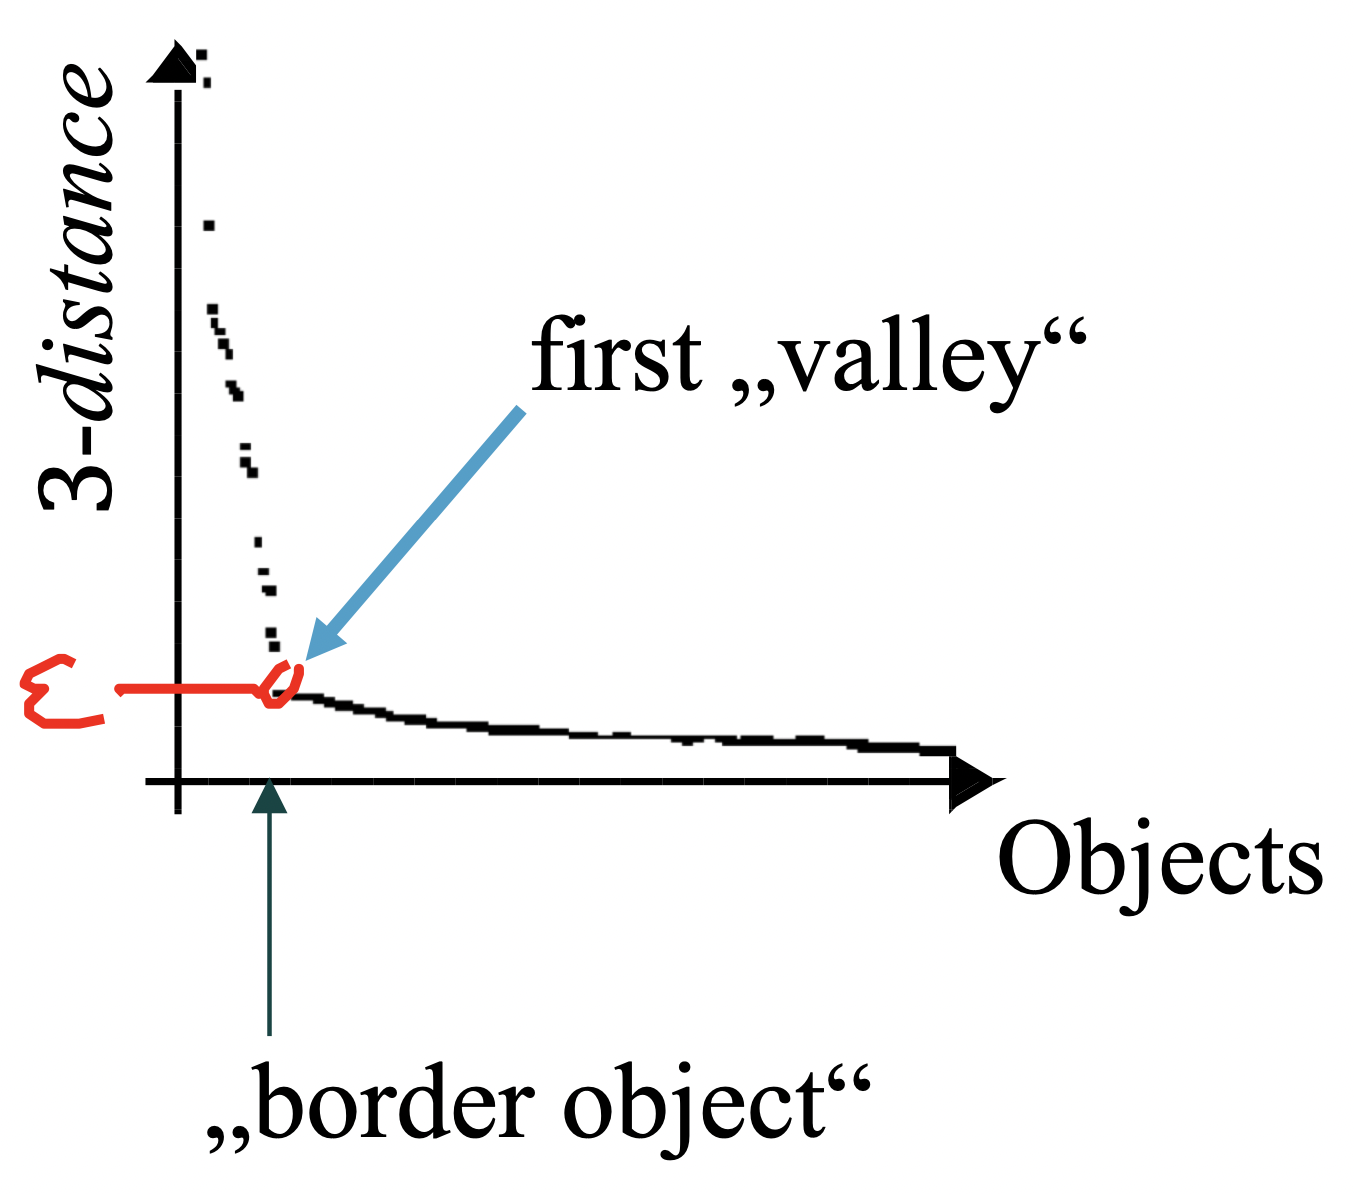
\includegraphics[width=0.3\textwidth]{images/valley.png}
    \end{center}
    
    The heuristic is then as follows:
    \begin{itemize}
        \item Fix a value for minpts (default is $2d - 1$), where $d$ is the dimension
        \item User selects ``border object'' $o$ from the minpts distance plot, $\varepsilon$ is set to minpts\-distance $o$.
    \end{itemize}
    
\subsubsection{Advantages and disadvantages of DBSCAN}
    The advantages are 
    \begin{itemize}
        \item Does not require to specify number of clusters
        \item Performs well with clusters of arbitrary shape
        \item DBSCAN is robust to outliers and is able to handle them
    \end{itemize}
    The disadvantages are
    \begin{itemize}
        \item It requires domain knowledge and it is not easy to determine $\varepsilon$
        \item If clusters are very different in terms of in-cluster densities, then DBSCAN is not well suited to define clusters. DBSCAN cannot generalise well to clusters with very different densities
    \end{itemize}
    
\subsection{DENCLUE}
    DENCLUE gets rid of annoying $\varepsilon$ and minpts.
    
    The idea behind DENCLUE is to generalise the notion of neighbourhood density by considering overall density distribution with density estimation techniques
    
    Density estimation is to 
    \begin{itemize}
        \item Determine the unknown probability density function
        \item It is non-parametric and does not assume a fixed probability model
        \item Tries to determine the probability density at each point
        \item DBSCAN actually uses a simplified version of this idea
    \end{itemize}
    
\subsubsection{Density estimation}
There is a strong connection between density-based clustering and density estimation. 

Kernel density is a non-parametric technique that infers density at each point. Non-parametric means there is no fixed probability model.

\subsubsection{Univariate density estimation}
    In one dimension, we can model the data as a random variable $X$. Data points are observations $\set{x_1, \dots, x_n}$. We can estimate the CDF by counting how many points are $\leq x$. 
    \m{
        \hat{F}(x) = \frac{1}{n}\sum_{i=1}^{n}I(x_i \leq x)
    }
    Where $I$ is the indicator functions (Think boolean function that computes the predicate).
    
    The density function is then estimated by taking the derivative (recall shrinking secant definition of derivatives)
    \m{
        \hat{f}(x) = \frac{
        \hat{F}(x + \frac{h}{2}) - \hat{F}(x - \frac{h}{2})
        }{h} = \frac{k/n}{h} = \frac{k}{nh}
    }
    Here $k$ is the number of points in the window of width $h$ centered on $x$. The density estimate is ratio of points in the window $(k/n)$ to the volume of the window $h$.
    
\subsubsection{Kernel density estimation}
    The idea behind kernel density estimation is to use a kernel function $K$ which is non-negative, symmetric and integrates to $1$. So $K(x) \geq 0, K(-x) = K(x)$ and $\int{K(x) dx = 1}$.
    
    The discrete kernel is 
    \m{
    K(z) = \begin{cases} 
                1 & \text{if } |z| \leq \frac{1}{2} \\
                0 & \text{otherwise}
    \end{cases}
    }
    Where $|z| = \frac{x - x_i}{h}$ for a window width $h$. This is basically just a probability distribution function.
    
    We can rewrite the density estimator as 
    \m{
        \hat{f}(x) = \frac{1}{nh} \sum_{i=1}^{n}K(\frac{x-x_i}{h})
    }
    Where 
    \m{
        z = \frac{x- x_i}{h} \leq \frac{1}{2}
    }
    Was used in the derivation.
    This method is not discrete however, so we can use a Gauss kernel (which is smooth). This is the underlying model behind DBSCAN. Data points within the neigborhood range contribute fully, and those outside not at all. 
    
    DENCLUE uses the Gauss kernel as given by
    \m{
        K(z) = \frac{1}{\sqrt{2\pi}} e(-\frac{z^2}{2)}
    }
    
    This makes our kernel
    \m{
        K(\frac{x - x_i}{h}) = \frac{1}{\sqrt{2\pi}} exp(-\frac{(x- x_i)^2}{2h^2})
    }
    Where $x$ at the center of the window plays the role of the mean, and $h$ the standard deviation. 
    
\subsubsection{Multivate density estimation}
    For $d$-dimensional data, the window is a hypercube centered at $x$ with volume $h$, that is $vol(H_d(h)) = h^d$. Density estimation is the same as before, except now it is the fraction of point weight within window, divided by volume. 
    
    \m{
        \hat{f}(x) = \frac{1}{nh^d}\sum_{i=1}^{n}{K(\frac{x-x_i}{h})}
    }
    The multivariate kernel still has to integrate to $1$. 
    
    Discrete kernels are almost as before, except
    \m{
    K(z) = \begin{cases} 
                1 & \text{if } |z| \leq \frac{1}{2} \text{for all dimensions} \\
                0 & \text{otherwise}
    \end{cases}
    }
    The Gaussian kernel is (with $I = \Sigma$ covariance matrix)
    \m{
        K(z) = \frac{1}{(2\pi)^{\frac{d}{2}}} \exp(-\frac{z^Tz}{2})
    }
\subsubsection{Nearest neighbor estimation}
    Kernel density estimation is
    \begin{itemize}
        \item Fix volume $h$ of dense region
        \item Kernel function finds the number or weight of points inside the region with fixed volume
    \end{itemize}
    $k$-nearest neighbour is
    \begin{itemize}
        \item Fix $k$, the number that defines a dense region
        \item The volume varies with $k$
        \item Given $k$, estimate density at $x$ as \m{
            \hat{f}(x) = \frac{k}{n\cdot vol (S_d(h_x))}
        }
    \end{itemize}
    Here $h_x$ is the distance from $x$ to its $k$-nearest neighbour. The volume is the volume of the $d$-dimensional hypersphere centered at $x$. 
    
\subsubsection{DENCLUE: Density attractors}

A set of $C$ of data points from a data set $D$ is a density-based cluster w.r.t to some threshold $\chi$ if there exists a set of attractors $x_1^*, \dots, x_m^*$ if 
\begin{itemize}
    \item Each point $x$ in $C$ is attracted to some attractor $x_i^*$
    \item Each density attractor $x_i^*$ exceeds some density threshold $\chi : \hat{f}(x_i^*) \geq \chi$
    \item Any two density attractors $x_i^*, x_j^*$ are density reachable. That is, there exists a path from $x_i^*$ to $x_j^*$ such that for all points $y$ on the path, $\hat{f}(y) \geq \chi$
\end{itemize}

The DENCLUE algorithm works as follows:
\begin{enumerate}
    \item $A = \emptyset$
    \item Foreach $x \in D$ (Find density attractors)
    \item $x^* = FindAttractor(x, D, h, \varepsilon$
    \item If $\hat{f}(x^*) \geq \chi$ then $A = A \cup \set{x^*}$, and $R(x^*) = R(x^*) \cup \set{x}$
    \item endif
    \item $C' = \set{maximal C \subseteq A | \forall x_i^*, x_j^* \in C, x_i^*, x_j^* density reachable}$
    \item Foreach $C \in C'$ and foreach $x^* \in C$ let $C = C \cup R(X^*)$ (Density-based clusters)
    \item Return $C$
\end{enumerate}
Finally, the FindAttractor function is as follows
\begin{enumerate}
    \item $t = 0$
    \item $x_t = x$
    \item Repeat 
    \m{
        x_{t+1} = \frac{\sum_{i=1}^{n}K(\frac{x_t - x_i}{h})}{\sum_{i=1}^{n} K(\frac{x_t - x_i}{h})}}
    And \m{
        t = t + 1
    }
    \item Until $||x_t - x_{t-1}|| \leq \varepsilon$
    \item Return $x_t$
\end{enumerate}
It runs in $O(n^2t)$ where $t$ is the number of iterations.

\subsubsection{MISSING: What are density attractors?}
    
\subsubsection{Advantages and disadvantages of the DENCLUE algorithm}
    DBSCAN corresponds to discrete kernel, which is more efficient. DENCLUE uses Guassian kernel density based attractors, which is a smooth model. 
    The advantages are 
    \begin{itemize}
        \item Clusters can arbitrary shape and size, clusters are not restricted to have convex shapes
        \item Number of clusters is determined automatically
        \item Can separate clusters from surrounding noise
        \item Can be supported by spatial index structures
    \end{itemize}
    The disadvantages are
    \begin{itemize}
        \item Input parameters may be difficult to determine
        \item Can be sensitive to input parameter setting
    \end{itemize}
    
\subsection{Incremental clustering}
    If new data points arrive, then we need to update our algorithms so that they can be made incremental.
    
\subsubsection{Incremental DBSCAN}
    In density based clustering, only a certain neighborhood is affected by insertion and deletion, and therefore it is not necessary to recluster the entire database. For example, in insertion, we only have 4 cases, and therefore we only need to check the effected $\epsilon$-neighbourhood. 
    
       
    \begin{center}
        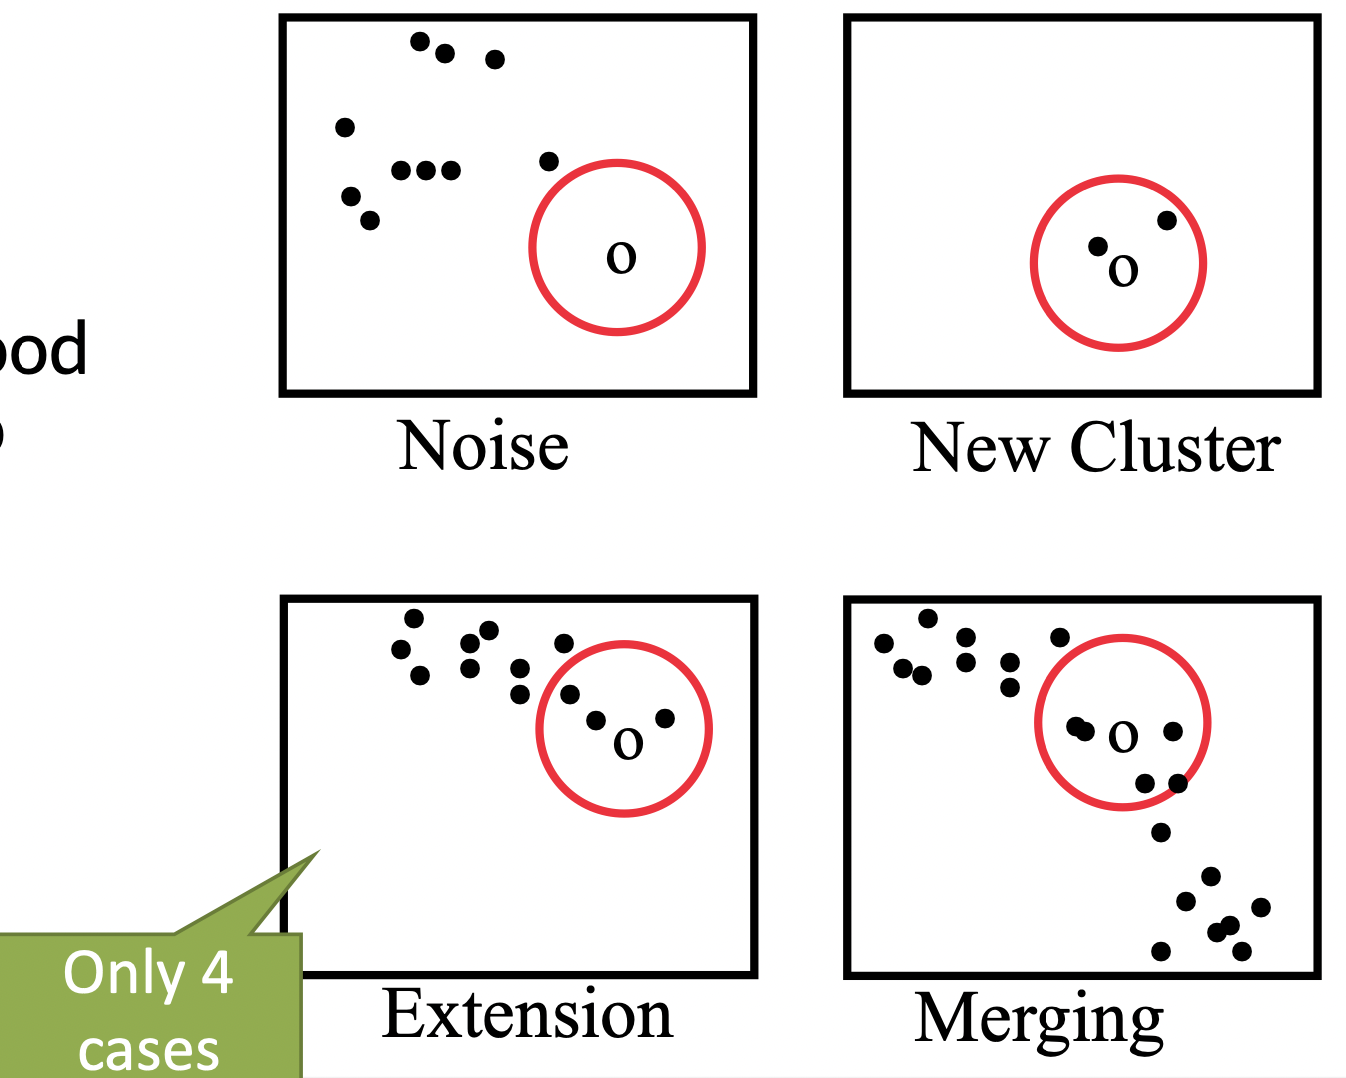
\includegraphics[width=0.5\textwidth]{images/4cases.png}
    \end{center}
    
    We only need to look for points in the $\varepsilon$-neighbourhood of objects that core in order to update.